\section{Experiments}
%In this section, we present the experiments of LPAF for language model compression. We compare with state-of-the-art compression methods and perform detailed analysis of the results to provide guidance under different resource budgets.
\subsection{Datasets}
We evaluate our approach on the following tasks: Stanford Sentiment Treebank~(SST-2)~\cite{sst2} which is 
a binary sentiment classification task,
Quora Question Pairs~(QQP) which is a paraphrase similarity matching task,
Multi-Genre Natural Language Inference~(MNLI)~\cite{mnli} and QNLI, which are two NLI tasks, 
and finally SQuAD v1.1~\cite{qnliandsquad} which is an extractive 
question answering task. All except the last one use accuracy as the evaluation metric, while SQuAD
uses the F1 score.

Following previous work~\cite{pkd,theseus}, we evaluate under a task-specific setting, i.e., we utilize no external corpus but only assume access to the training data of each task.


\subsection{Experimental Setup}
 \paragraph{Baselines}
 DistilBERT~\cite{distilbert}, PD-BERT~\cite{pdbert}, and  TinyBERT~\cite{tinybert} are  task-agnostic distillation methods involving a pre-training compression stage using unlabeled corpus; BERT$_\text{Truncated}$ directly fine-tunes a truncated BERT model; Vanilla KD uses vanilla Knowledge Distillation~\cite{kd}; PKD~\cite{pkd} introduces patient distillation for intermediate feature matching; RAIL-KD~\cite{rail} randomizes the layer mapping which is fixed in PKD; Theseus~\cite{theseus} proposed a new genere of model compression by progressive module replacing; CKD~\cite{CKD} utilizes a novel KD objective to transfer the contextual knowledge via word relation and layer transforming relation; MetaDistil~\cite{metadistil} introduces meta-learning for training the teacher to better transfer knowledge to the student; SVD~\cite{svd} applies standard singular value decomposition on densely fine-tuned model and re-trains the decomposed model. We  compare with model architecture-dependent structured pruning~\cite{l0} in Appendix \ref{sec:appendixC}.

\paragraph{Training Details}
We obtain the results of baselines by running their official implementations. For LPAF, we tune the pruning hyper-parameter $\tau$ such that $T_{sparse}$ retains at least 97\% performance of densely fine-tuned BERT. We search $p_{init}$ in \{0.7, 0.5, 0.3\} and decay it to zero after half of the total training steps. We discuss the influence of different $p_{init}$ in \secref{sec:analysis}. During training, we
fix the batch size to 32 to reduce the search space. The max input length is set to 384 for SQuAD and 128 for other tasks. We use the AdamW~\cite{adamw} optimizer and search learning rate in \{2e-5,3e-5\}. The training epochs are set to 6. We report the results on the test set for SQuAD and the development set for other tasks. 
%All experiments are conducted on an RTX 2080Ti GPU with 12GB RAM.

\paragraph{Compression Setting}

We compress a 86M parameter BERT-base model  into compact models of various sizes. 
We refer to BERT-base compressed by  LPAF with preserved rank $k$ as LPAF-$k$ throughout \secref{sec:main} and \secref{sec:analysis}. We select $k$ from \{120,100,80,60,40\}, which corresponds to about \{22\%,19\%,15\%,12\%,8\%\} of original parameters. In addition, we also report FLOPs to measure the computation cost based on the number of floating-point operations for processing one sample.

 All baselines except for SVD achieve different compression rates by varying the number 
of encoder layers, hence comparison under the exact same model size is infeasible. 
We therefore set the number of layers in these baseline models to \{3, 2, 1\}, 
which corresponds to \{25\%, 16\%, 8\%\} of BERT's parameters. 
This makes their model sizes and FLOPs roughly equal to those of SVD/LPAF-120/80/40. 
SQuAD needs higher FLOPs than other tasks given the same  rank $k$ due to its longer input  length. See \tabref{table:stats} for details.

\begin{table}[th]
	\scriptsize
	\centering
	\begin{tabular}{l|cc|cc}
		\toprule
		Task& \multicolumn{2}{c|}{Others} & \multicolumn{2}{c}{SQuAD v1.1} \\
		\midrule
		Metric & \% of Param.           & FLOPs               & \% of Param.      & FLOPs        \\
		\midrule
		BERT-base & 100               & 7.4G                & 100        & 35.4G        \\
		\midrule
		LPAF-120   & 22       & 1.9G          & 22  & 10.3G  \\
		LPAF-100   & 19      & 1.6G          & 19  & 9.1G   \\
		LPAF-80    & 15       & 1.3G          & 15  & 7.9G   \\
		LPAF-60    & 12        & 1.0G         & 12  & 6.6G   \\
		LPAF-40    & 8        & 0.7G        & 8  & 5.3G \\ 
		\bottomrule
	\end{tabular}
	\caption{Percentage of parameters and FLOPs.}
	\label{table:stats}
\end{table}


\subsection{Main Results}
\label{sec:main}
%We present the experimental results of LPAF with different compression rate as well as overall comparison with state-of-the-art baselines.
\subsubsection{Comparisons with different $k$}

\begin{table}[h]
	\centering
	\scriptsize
	\begin{tabular}{l|ccccc}
		\toprule
		Model & SST-2 & QNLI & MNLI & QQP  & SQuAD v1.1 \\
		\midrule
		BERT-base &92.0 &91.4 &84.0 &92.4 &88.4 \\
		$T_{sparse}$     & 89.7  & 89.2 & 82.0 & 90.1 & 87.0  \\
		\midrule
		LPAF-120 & 90.7  & 89.2 & 82.1 & 90.4 & 87.2  \\
		LPAF-100 & 90.3  & 88.8 & 82.0 & 90.2 & 86.6  \\
		LPAF-80  & 89.7  & 88.6 & 81.4 & 90.1 & 85.7  \\
		LPAF-60  & 88.8  & 87.3 & 80.5 & 89.7 & 84.4  \\
		LPAF-40  & 88.5  & 85.7 & 79.2 & 89.0 & 82.0 \\
		\bottomrule
	\end{tabular}
	\caption{Experimental results~(average of 3 runs) of different LPAF-$k$.}
	\label{table:diffk}
\end{table}


%\begin{figure*}[t]
%	\centering
%	\scalebox{0.164}{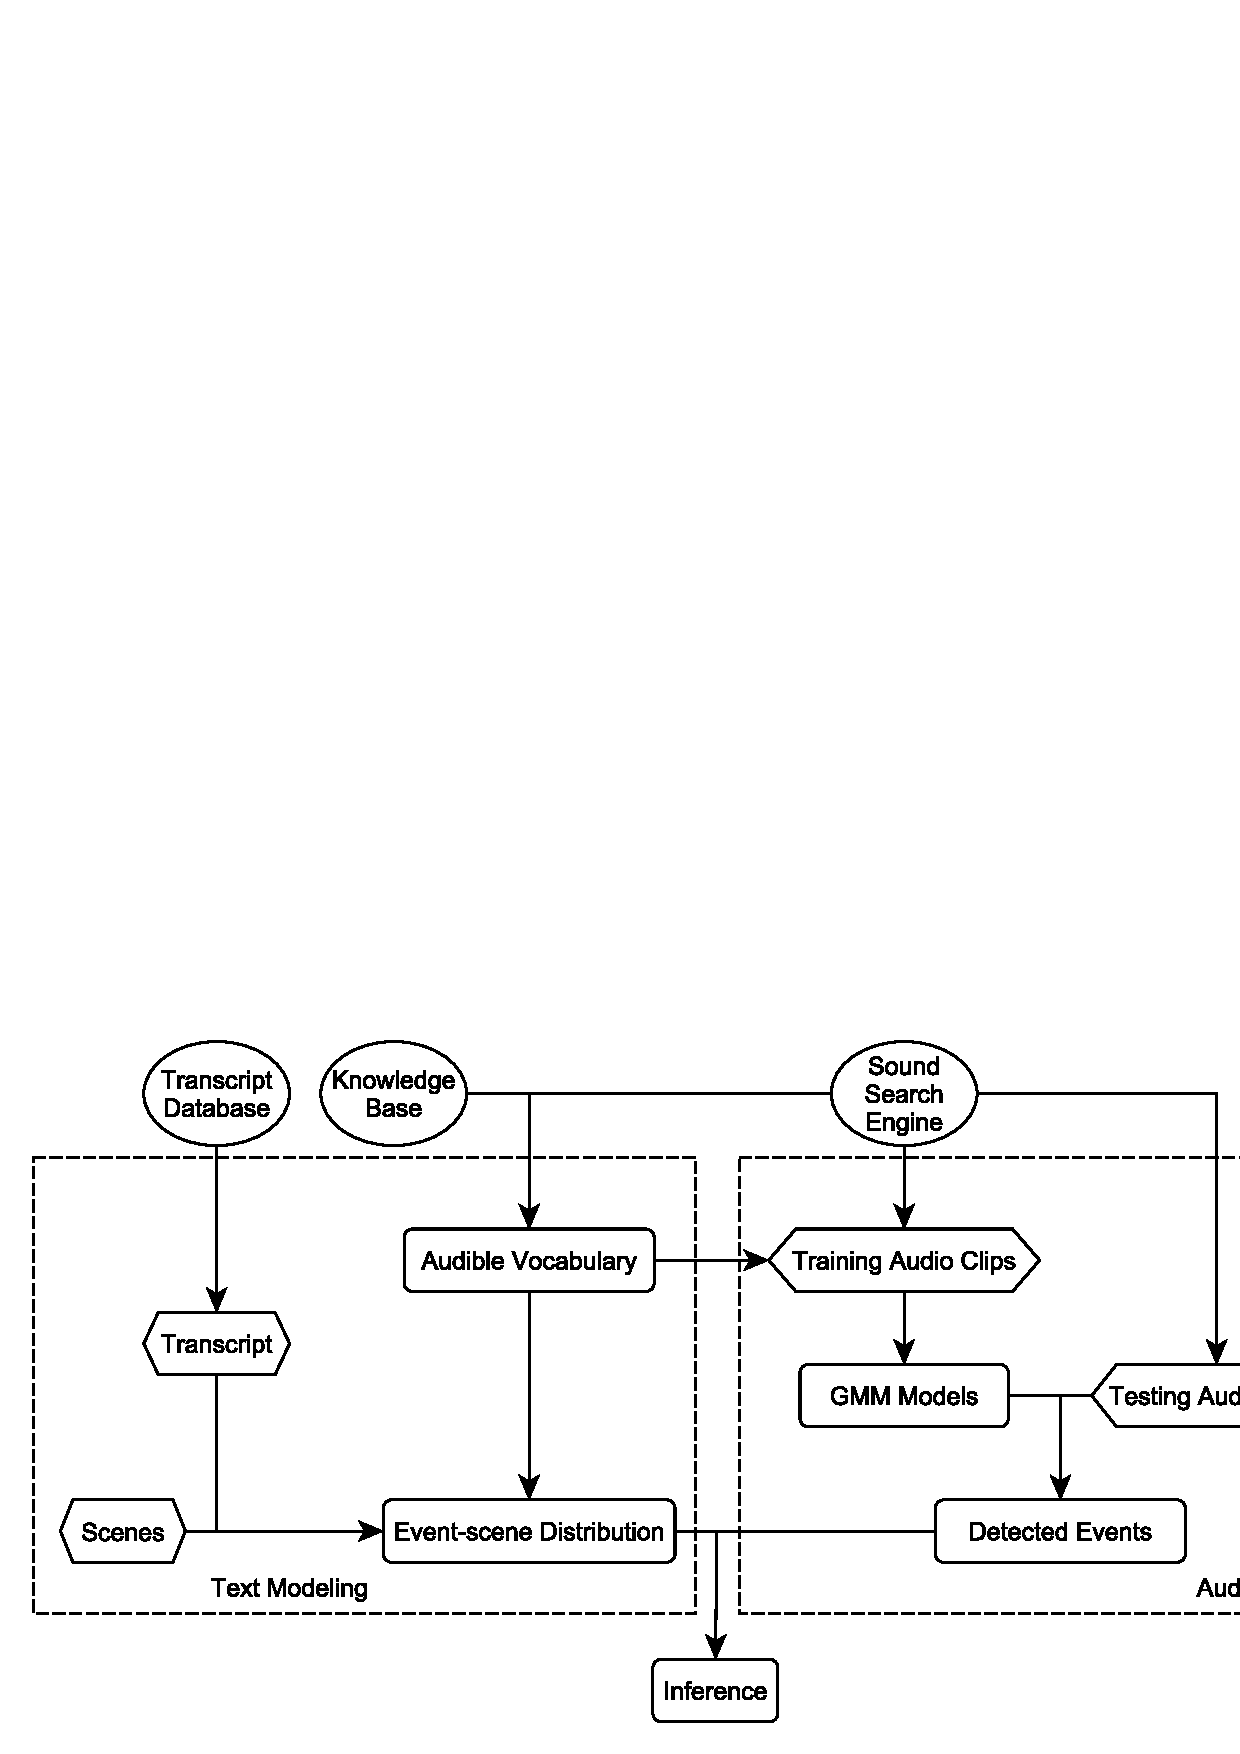
\includegraphics{./figures/all.pdf}}
%	\caption{Experimental results~(average of 3 runs) of our proposed LPAF and all compared baselines. We use the horizontal gray line to indicate the performance of $T_{sparse}$ for reference purpose.} 
%\label{fig:all}
%\end{figure*}

	\begin{table*}[thb!]
	\centering
	\scriptsize
	\begin{tabular}{l|c|ccccc}
		\toprule
		Task &Type  & SST-2~(67K)                                                  & QQP~(364K)                                                    & QNLI~(105K)                                                   & MNLI-m/mm~(393K)                                                   & SQuAD v1.1~(88K)                                             \\
		\midrule
		 Test Metric&-  & Accuracy                                                  & Accuracy                                                    & Accuracy                                                   & Accuracy                                                   & F1 Score                                            \\
		\midrule 
		\% of \#Param.~$\downarrow$ &- &25\% ~16\%  ~~8\%            &25\% ~16\%  ~~8\%             &25\% ~16\%  ~~8\%            &25\% ~~~~~~~~~	~16\%  ~~~~~~~~~~8\%            &25\% ~16\%  ~~8\%            \\
		\midrule
%			 \multicolumn{6}{c}{\textit{Task-agnostic Distillation}}   \\
%			\midrule
		DistilBERT    &\multirow{3}{*}{\minitab[c]{\textit{Task-agnostic} \\ \textit{Distillation}}}  & 88.9 ~86.4 ~83.0          & 89.4~ 88.0~ 82.4          & 83.8~ 81.6~ 64.9          & 76.4/76.4 ~71.6/70.9 ~59.8/58.6          & 78.0~ 66.5 ~28.5          \\
		PD-BERT    &     & 88.2~ 87.5~ 82.7          & 89.8 ~88.9 ~82.9          & 86.1~ 83.4~ 65.9          & 78.6/78.3 ~75.9/75.9 ~66.0/65.9          & 77.0 ~45.2~ 22.8          \\
		TinyBERT    &    & 89.8 ~88.0 ~82.6          & 90.0~ 88.7~ 83.2          & 87.7 ~84.5~ 63.1          & 80.6/80.5~ 77.1/77.7~ 65.6/66.2          & 58.0 ~38.1 ~15.4          \\
\midrule
%\multicolumn{6}{c}{\textit{Task-specific Distillation}}   \\
%\midrule
		BERT$_{\text{Truncated}}$ &\multirow{7}{*}{\minitab[c]{\textit{Task-specific} \\ \textit{Distillation}}}  & 87.7 ~85.6 ~79.6          & 88.0~ 86.9 ~82.2          & 83.0 ~78.7 ~60.3          & 75.7/73.2~ 73.1/72.3~ 60.6/60.3          & 54.8~ 31.4~ 17.1          \\
		Vanilla KD     &    & 88.5~ 86.5 ~82.0           & 88.8~ 87.2 ~82.3          & 83.6 ~78.6~ 59.8          & 76.1/73.5 ~73.3/72.6~ 61.3/61.2          & 62.5 ~32.3~ 17.0          \\
		PKD    &    & 88.1~ 87.2 ~82.0          & 88.5~ 87.5 ~82.3          & 82.7~ 78.0~ 59.8          & 75.8/75.6 ~73.0/72.3~ 61.3/61.2          &60.5~ 31.5~ 17.0                                                      \\
		Theseus &  & 88.5~ 86.1~ 79.6          & 89.0 ~86.0 ~82.2          & 85.0 ~80.3~ 60.3          & 76.3/76.4~ 73.4/73.6 ~60.6/60.3          &72.7~ 63.2~ 26.2                                                      \\
		RAIL-KD     &   & 88.8~ 86.8~ 83.9          &\underline{90.2} ~88.6 ~\underline{83.3}          &85.7 ~81.2~ 65.7          &78.8/78.8 ~73.5/74.0 ~62.1/61.4          &78.7~ 69.5~ 32.1                                                      \\
		CKD   &     & \underline{89.8} ~\underline{88.7}~ 84.1          & 90.1~ \underline{88.9}~ 82.9          & \underline{87.0}~ \underline{84.9} ~67.6          & 79.1/78.9 ~\underline{76.8}/76.8~ 66.4/66.7          &78.9~ 69.1~ 33.1                                                      \\
		MetaDistil  &      & 88.9 ~87.0~ 82.7          & 88.9~ 86.9~ 82.1          & 86.8~ 84.9 ~67.5          & 79.2/79.7 ~76.7/\underline{77.0}~ 66.4/66.7          &78.8~ 69.0~ 32.4                                                      \\
		\midrule
% \multicolumn{6}{c}{\textit{Factorization-based}}   \\
%\midrule
		SVD   &\multirow{2}{*}{\minitab[c]{\textit{Matrix} \\ \textit{Factorization}}}    & 88.9 ~88.1~ \underline{84.5}         & 90.0 ~87.9~ 83.1          & 86.1 ~83.8~ \underline{67.6}          & \underline{79.6/80.2}~ 76.6/76.7~ \underline{71.6}/\underline{72.2}          & \underline{85.5}~ \underline{81.1}~ \underline{51.3}          \\

		LPAF~(ours)   &     & \textbf{90.7~ 89.7~ 88.5} & \textbf{90.4}~ \textbf{90.1}~ \textbf{89.0} & \textbf{89.2~ 88.6~ 85.7} & \textbf{82.2/82.9}~ \textbf{81.4/81.9}~ \textbf{79.2/80.1} & \textbf{87.2 ~85.7 ~82.0} \\
		\bottomrule
	\end{tabular}
	\caption{Experimental resutls~(average of 3 runs) of different methods for compressing BERT-base into smaller ones with various sizes. The best results are \textbf{bolded} and the second best are \underline{underlined}. The numbers in the parenthesis are training data size for each task.}
	\label{table:all}
\end{table*}




\tabref{table:diffk} shows the results of LPAF with various preserved rank $k$. 
Compared to densely fine-tuned BERT, $T_{sparse}$ inevitably shows a slight performance drop 
on all tasks with an average sparsity of 86.3\%.
Comparing \tabref{table:diffk} with \tabref{table:pilot}, we can see that LPAF consistently outperforms SVD under every choice of $k$ by a large margin. The improvement is more evident under a high compression regime. For example, LPAF-40 outperforms SVD-40 by 15.2 percentage 
points on QNLI and 5.9 points on QQP, respectively. Overall, LPAF shows much strong 
compression performance than SVD, demonstrating the importance of a 
low-rank structure for factorization.


\subsubsection{Comparisons with Baselines}
\tabref{table:all} summarizes the overall results. Not surprisingly, BERT$_{\text{Truncated}}$ performs the worst on all tasks. Among task-specific distillation methods, CKD shows the best overall performance thanks to its better initialization using PD-BERT and the use of a sophisticated distillation objective. Task-agnostic distillation methods generally outperform task-specific distillation methods except for CKD, showing that a pre-training compression stage is helpful when the compression rate is high. SVD shows an obvious advantage over other baselines under a high compression rate. This is because when the models are too shallow, i.e.,  less than 3 layers, the model capacity becomes insufficient. In contrast, SVD reduces model size at the matrix level while keeping the number of layers unchanged. Under all compression ratios, LPAF consistently gives the best results, verifying its general effectiveness. For extreme compression rate, e.g., 8\%  on SST-2, LPAF shows large advantage by retaining 96.2\% and 98.6\% of the performance of fine-tuned BERT and $T_{sparse}$. On the SQuAD dataset where more complex reasoning is needed, LPAF shows up tp 30.2 points improvement over SVD, demonstrating its superiority on linguistic tasks beyond sentence classification.

\subsection{Analysis}
\label{sec:analysis}
\paragraph{Effect of different $T_{sparse}$} 
Recall that we choose the low-rank sparse model $T_{sparse}$ with at least 97\% of the fine-tuned BERT's performance. Here we experiment with different $T_{sparse}$ by altering threshold $\tau$ and examine its effect on the performance of LPAF \textit{without} sparsity-aware SVD and mixed-rank fine-tuning.
% \KZ{Why experiment with QNLI here while test with SST-2 for the next two subsections? Some people might be suspecting 
%something fishy.}
The results on SST-2 are summarized in \tabref{table:diffsparse}. As we increase $\tau$, $T_{sparse}$ becomes more sparse and its rank also monotonically decreases. We observe that for a fixed $k$, the performance of LPAF-$k$ turns out to resemble a unimodal distribution of the rank of $T_{sparse}$: as the rank gets too high, the increased approximation error overturns the benefit of improved accuracy; when the rank is too low, the drop of accuracy also overturns the benefit of decreased approximation error. Generally, the best performance of LPAF-$k$ for a larger $k$ is achieved at a higher rank of $T_{sparse}$ compared to that of a smaller $k$.
%\KZ{This suggests that LPAF should be used at a $k$ compatible with the $k$ of the $T_{sparse}$?}
% Please add the following required packages to your document preamble:
% \usepackage{multirow}
\begin{table}[t]
	\centering
	\scriptsize
	\begin{tabular}{l|llll}
		\toprule
		&	\multicolumn{4}{c}{$T_{sparse}$} \\
		\midrule
		\multicolumn{1}{l|}{$\tau$~~~~~~~~~~~~~~~~~~~~~~~~$~~~~~\uparrow$}           &65  &90  &180           &310                      \\
				 \multicolumn{1}{l|}{\% of Param.~~~~~~~~~~~~~$\downarrow$}           & 30\% & 25\% & 16\%          & 10\%                     \\
		\multicolumn{1}{l|}{Rank~~~~~~~~~~~~~~~~~~~~~$~~\downarrow$}               &545   &471   &349            &294                        \\
		\multicolumn{1}{l|}{Accuracy~~~~~~~~~~~~~~$~~\downarrow$}           & 90.9 & 90.3 & 89.1          & 88.2                     \\

		\midrule
		\multicolumn{1}{l|}{$k$=120}       &\textbf{90.1}  &89.5  &89.0           &88.6                      \\
		\multicolumn{1}{l|}{$k$=100}        &88.8  &\textbf{89.5}  &88.4           &88.4                      \\
		\multicolumn{1}{l|}{$k$=80}                  &87.2  &\textbf{89.3}  &88.2  &87.4                      \\
		\multicolumn{1}{l|}{$k$=60}                  &87.1  &87.3  &88.0           &\textbf{88.2}             \\
		\multicolumn{1}{l|}{$k$=40}                  &85.1  &85.3  &85.8           &\textbf{87.2}             \\
		\bottomrule
	\end{tabular}
	\caption{Effect of using different $T_{sparse}$ on SST-2.
}
	\label{table:diffsparse}
\end{table}


\paragraph{Effectiveness of sparsity-aware SVD}
In our sparsity-aware SVD, the reconstruction error of each parameter $\bm{W}_{i,j}$ is weighted by its importance score $\bm{S}_{ij}$. To examine its effectiveness in factorizing sparse matrix, we experiment with two variants on SST-2 dataset: (1) $\bm{S}$ is replaced by coarse-grained binary score $\bm{M}$; (2) non-weighted vanilla SVD. \tabref{table:diffsvd} shows that weighting by importance score yields the best results under all $k$, and a simple binary weighting strategy using $\bm{M}$ also brings improvement compared to vanilla SVD. This means that our sparsity-aware SVD is still applicable even when $\bm{S}$ is unavailable.
\begin{table}[th]
	\centering
	\scriptsize
	\begin{tabular}{l|lllll}
		\toprule
		Weighting Strategy         &$k$=120  & $k$=100  & $k$=80   & $k$=60   & $k$=40   \\
		\midrule
		- w/ $\bm{S}$    &\textbf{89.5}  & \textbf{89.4} & \textbf{88.8} & \textbf{88.4} & \textbf{87.9} \\
		- w/ $\bm{M}$   &89.1   & 88.9 & 88.5 & 88.3 & 87.4 \\
		- w/o $\bm{S}$ or $\bm{M}$ &88.8 & 88.7 & 88.0 & 87.4 & 87.1 \\
		\bottomrule
	\end{tabular}
	\caption{Ablation study on different weighting strategies for SVD on SST-2.}
	\label{table:diffsvd}
\end{table}


As stated in \secref{sec:sasvd}, we expect sparsity-aware SVD to retain more task performance from $T_{sparse}$ compared to vanilla SVD. We verify this by comparing their performances before fine-tuning. 
\figref{fig:init} shows that by informing the matrix factorization process with sparsity, 
more task performance can be retained at the beginning. 
Also, weighting by importance score gives slightly better initial performance due to 
its finer granularity.
\begin{figure}[th]
	\centering
	\scalebox{0.276}{\includegraphics{./figures/init.pdf}}
	\caption{Performance of $T_{factorized}$ on SST-2 with different factorization methods before fine-tuning.}
	\label{fig:init}
\end{figure}

\paragraph{Effectiveness of mixed-rank fine-tuning} In \tabref{table:wwomixedrank}, we examine the effectiveness of mixed-rank fine-tuning by ablation study.  Results show that mixed-ranking fine-tuning consistently brings improvement over standard fine-tuning under all choices of $k$. Adding the consistency objective $\mathcal{L}_{c}$  stabilizes training and leads to further improvement. 
\begin{table}[th]
	\centering
	\scriptsize
	\begin{tabular}{l|lllll}
		\toprule
		Fine-tuning Method & $k$=120 & $k$=100 & $k$=80 &$k$=60 & $k$=40 \\
		\midrule
		mixed-rank      & \textbf{90.7}  & \textbf{90.3}  & \textbf{89.7} &\textbf{89.0}  & \textbf{88.5} \\
		- w/o $\mathcal{L}_{c}$    &89.8 &89.6   &89.1  &88.5 &88.1  \\
		\midrule
		vanilla  & 89.5  & 89.4  &88.8  &88.4 & 87.9	 \\
		\bottomrule
	\end{tabular}
	\caption{Ablation of mixed-rank fine-tuning on SST-2.}
	\label{table:wwomixedrank}
\end{table}

We also study the effect of using different values of $p_{init}$ on the performance of mixed-rank fine-tuning. From \tabref{table:diffp} we can see that: (1) for $T_{factorized}$ with smaller $k$, it prefers a relatively large $p_{init}$ because its model capacity is largely reduced and it can benefit more from mixed-ranking fine-tuning to improve generalization; (2) for $T_{factorized}$ with larger $k$, a smaller $p_{init}$ is more favorable because its higher capacity makes it less likely to converge into bad local minimum; (3) setting $p_{init}$ to zero makes our method degenerate to R-Drop, which loses certain regularization effect but still outperforms standard fine-tuning.
\begin{table}[th]
	\centering
	\scriptsize
	\begin{tabular}{cl|lllll}
		\toprule
		&     & $k$=120 & $k$=100 & $k$=80 & $k$=60 & $k$=40   \\
		\midrule
		\multirow{3}{*}{$p_{init}$} & 0.7 & 90.2  & 89.8  & \textbf{89.7} & \textbf{89.0} & \textbf{88.5} \\
		& 0.5 & 90.5  & \textbf{90.3}  & 89.5 & 88.8 & 88.3 \\
		& 0.3 & \textbf{90.7}  & 89.6  & 89.0 & 88.5 & 88.1 \\
		\midrule
		\multicolumn{2}{c|}{R-Drop~($p_{init}$=0.0)}     & 90.0  & 89.6  & 89.3 & 88.5 & 87.7 \\
		\bottomrule
	\end{tabular}
	\caption{Ablation study on different value of $p_{init}$ for mixed-rank fine-tuning on SST-2.
%	\KZ{If you reorg the $p_{init}$ in ascending order, you will see the bolded numbers organized in
%a diagonal pattern similar to Table 5. Does that suggest anything?}
}
	\label{table:diffp}
\end{table}


\subsection{Applicability to Other Models}
Our framework is model architecture-agnostic in that it operates purely on the 
matrix level throughout all stages. It is straightforward to apply LPAF to other pre-trained language models beyond BERT. To this end, we apply  LPAF to compress an already compact 12-layer and 384 hidden-dimmension MiniLMv2~\cite{minilm} with 21.5M parameters into even smaller ones with \{33\%, 25\%\} of original parameters. The results are shown in \tabref{table:roberta}. For LPAF, we observe a similar low-rank phenomenon~(281 on average) in the sparse model. The final model compressed by LPAF consistently outperforms those compressed by truncation, SVD and the strong distillation method CKD, showing its general applicability and effectiveness.

\begin{table}[h]
	\centering
	\scriptsize
	\begin{tabular}{c|ccc}
		\toprule
		Task & SQuAD v1.1   & QNLI     & MNLI-m/mm         \\
		\midrule
		 \% of \#Param. &33\%  ~~25\%            &~33\%  ~~25\%             &~33\%  ~~~~~~~~25\%          \\
		\midrule
	    Truncated       & 82.4 ~76.3          & 86.5~ 83.2          & 79.8/80.4~ 75.3/75.9         \\
	    CKD       & 83.7 ~77.8          & 87.2~ 83.3          & 80.0/80.6~ 75.4/76.0         \\

		\midrule
		SVD           & 83.1 ~78.2          & 86.0~ 83.5          & 80.3/81.0~ 77.5/78.6         \\
		LPAF~(ours)                  &\textbf{85.4} ~\textbf{83.9}          & \textbf{88.6}~ \textbf{87.8}          & \textbf{82.4/83.1}~ \textbf{81.5/82.3}           \\
		\bottomrule
	\end{tabular}
	\caption{Results~(average of 3 runs) of compressing MiniLMv2 into 33\%/25\% of original sizes.}
	\label{table:roberta}
\end{table}


